\section{Our Proposal}
\label{sec:proposal}

In this section we describe the architecture and functioning of our proposed User-Driven and Context-aware Hybrid Recommender System. Figure \ref{fig:arquitecture} shows its components:
\begin{itemize}
    \item \textbf{Data Gathering Module}: User preferences are received by the system, explicitly (direct interaction) or implicitly (data mining, social network analysis, etc.).
    \item \textbf{User Interest Module}: The preferences are propagated from higher classes to lower classes.
    \item \textbf{Context Module}: The system receives information about the context of the user, explicitly or implicitly (retrieved from an API, mobile information, etc.).
    \item \textbf{Recommendation Module}: The system recommends a set of places to the user.
\end{itemize}

In the following sections, we describe in detail each module.

\begin{figure}[h]
\centering
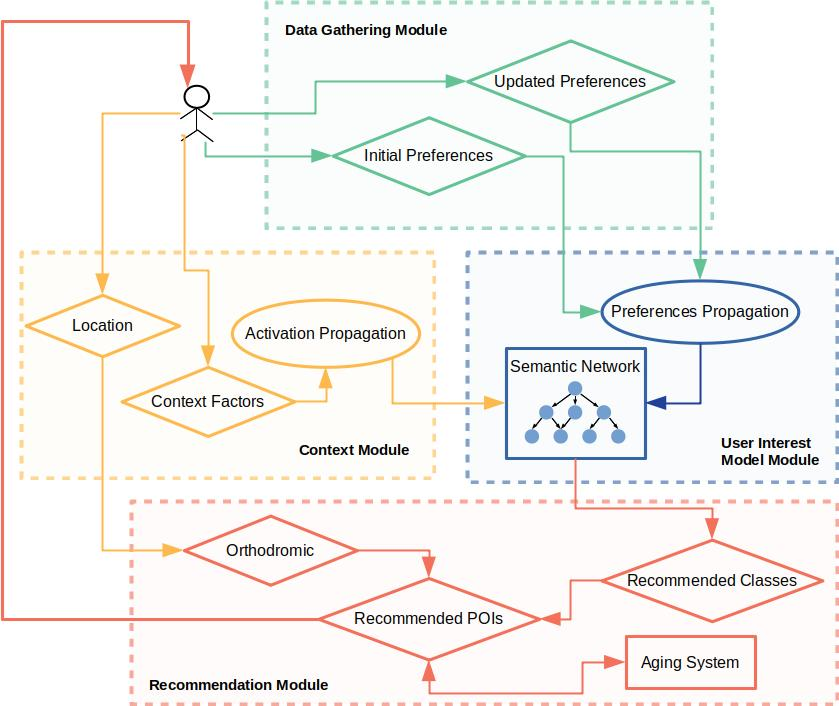
\includegraphics[scale=0.4]{draws/arquitecture.jpg}
\caption{System arquitecture}
\label{fig:arquitecture}
\end{figure}

\subsection{Data Gathering Module}
Initially, the system should receive initial \textbf{preferences}, as real values between $0$ and $1$, for the higher classes. To obtain these values, the user could explicitly set them by interacting with the system or they could be implicitly determined using data mining, social network analysis, geo-data, etc. During the lifetime of the system, the user can feed new updated preferences to the system.

\subsection{User Interest Model Module}
Inspired on the work of Bahramian et al. \cite{bahramian_abbaspour_claramunt_2017}, we introduce the concept of \textbf{semantic network}: a tourism ontology extended with the user's preferences (see figure \ref{fig:initial_pref}) and context factor links, a concept we explain later (see figure \ref{fig:init_act}). Just like Bahramian et al. \cite{bahramian_abbaspour_claramunt_2017}, we take advantage of the hierarchical shape of the semantic network for propagating the preference of superclasses to subclasses. Alongside preferences, each node of the semantic network has a \textbf{confidence} related to the user, a real value between $0$ and $1$ that defines how sure is the system that the computed preference is the real one. For computing the preference and the confidence we use formula \ref{eq:preference} and formula \ref{eq:confidence}, respectively:
\begin{equation} \label{eq:preference}
    pref_c = \frac{\displaystyle \sum_{p \in ancestors(c)}{conf_p pref_p}}
    {\displaystyle  \sum_{p \in ancestors(c)} {conf_p}}
\end{equation}
\begin{equation} \label{eq:confidence}
    conf_c = \frac{\displaystyle \sum_{p \in ancestors(c)} {conf_p}}{|ancestors(c)|} - \alpha
\end{equation}
where $ancestors(c)$ is the set of ancestors of the ontology class $c$, $pref_c$ is the preference of the class $c$, $conf_c$ is the confidence of the class $c$ and $\alpha$ is the \textit{decrease rate} that will tell how much should decrease the \textit{confidence} at each level. 

These formulas are applied to each node traversing from the higher classes, whose preferences are obtained from the Data Gathering Module, to the leaves. This process is called \textbf{preference propagation} and figures \ref{fig:initial_pref} and \ref{fig:pref_prop} show an example.

\begin{figure}[h]
\centering
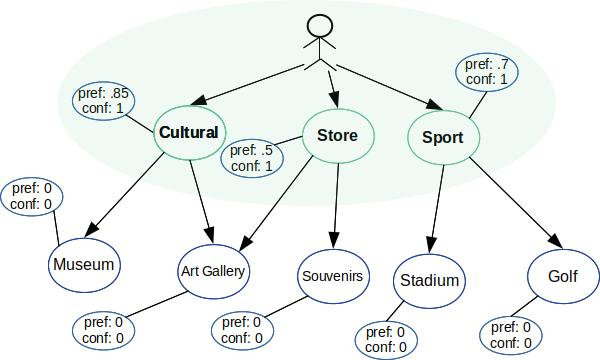
\includegraphics[scale=0.5]{draws/initial_pref.jpg}
\caption{Initial preferences for "Cultural", "Store" and "Sport" classes}
\label{fig:initial_pref}
\end{figure}

\begin{figure}[h]
\centering
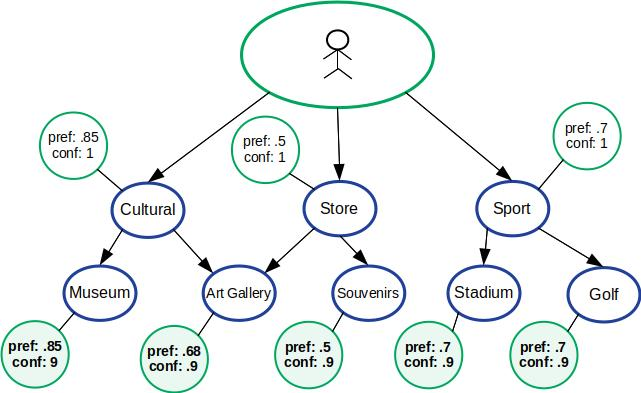
\includegraphics[scale=0.5]{draws/pref_spred.jpg}
\caption{Preference propagation for "Museum", "Art Gallery", "Souvenirs", "Stadium" and "Golf" classes, with decrease rate equal to 0.1}
\label{fig:pref_prop}
\end{figure}

\subsection{Context Module}
We define the \textbf{activation} of a node as the value that determines how feasible it is to go to a place that belongs to the node's ontology class in the current user's context. The user's context is determined by the \textbf{context factors}, entities that describe the characteristics of the user’s context that could affect their decision to go to a specific place. The context factors could be time, day and weather, as proposed by Bahramian \cite{bahramian_abbaspour_claramunt_2017}, but many others could be used, like transportation\cite{rajaonarivo2019rec} and mood. These entities are linked to the higher classes.

Let's define $f_x$ the \textit{fulfillment} of a context factor $x$ that has the value $1$ if $x$ fulfills or $0$ otherwise. Let's also define $r_{c,x}$ as the \textit{relevance} of context factor $x$ for node $c$, which is a real value in $[0, 2]$ that specifies how much the context factor can affect the decision to go to a POI that belongs to the node's ontology class; a value of $1$ means indifference; a value near $2$ means the fulfillment increases the wish to go to the POI; a value near $0$ means the fulfillment decreases the wish to go the POI. Hence, we define the activation for a node whose class $c$ is directly linked to the context factors:
\begin{equation} \label{eq:high_activation}
    act_c = \sum_{x \in contextFactors} r_{c,x} f_x
\end{equation}
and the activation for the internal nodes is defined as follows:
\begin{equation} \label{eq:activation}
    act_c = \frac{\displaystyle \sum_{c' \in ancestors(c)} act_{c'}}{|ancestors(c)|}
\end{equation}.
These formulas are used for an \textbf{activation propagation} from the higher classes. Figures \ref{fig:init_act}, \ref{fig:high_act} and \ref{fig:spread_act} show an example.

\begin{figure}[h]
\centering
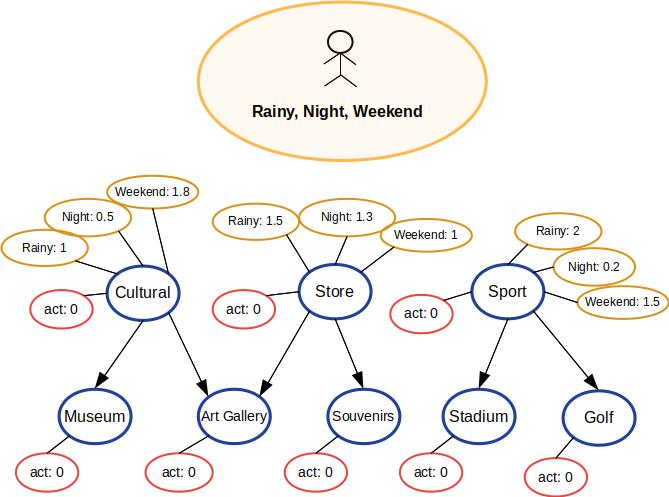
\includegraphics[scale=0.45]{draws/initial_act.jpg}
\caption{System receives (sunny, night, weekend) as user context}
\label{fig:init_act}
\end{figure}

\begin{figure}[h]
\centering
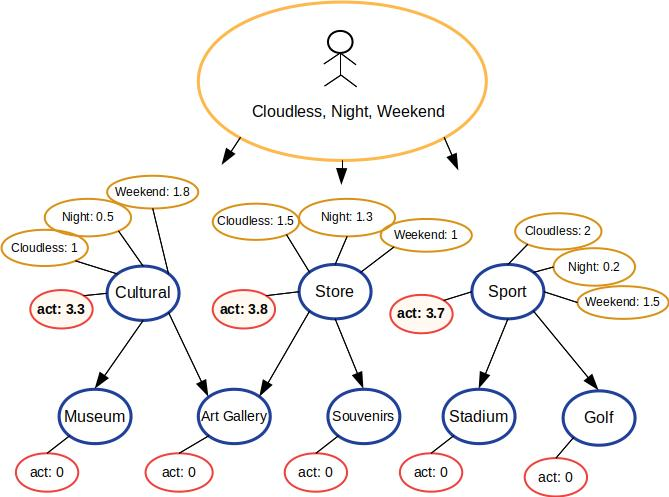
\includegraphics[scale=0.45]{draws/high_act.jpg}
\caption{Compute activation for "Cultural", "Store" and "Sport" classes}
\label{fig:high_act}
\end{figure}

\begin{figure}[h]
\centering
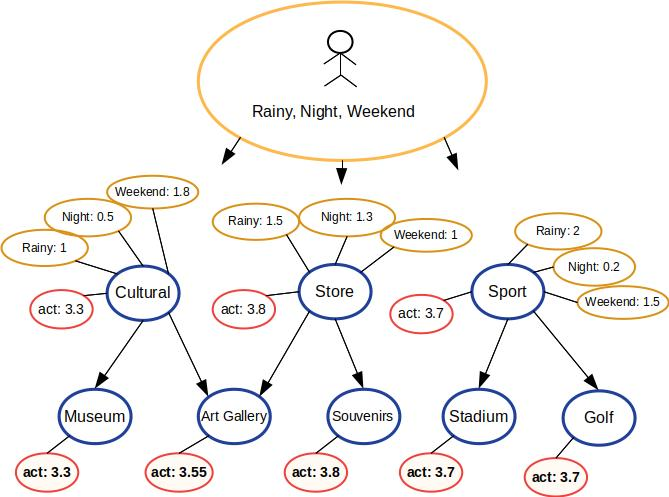
\includegraphics[scale=0.45]{draws/spread_act.jpg}
\caption{Spread activation to "Museum", "Art Gallery", "Souvenirs", "Stadium" and "Golf" classes}
\label{fig:spread_act}
\end{figure}

Furthermore, this module receives the user's \textbf{location}, which will be used for querying near POIs.

\subsection{Recommendation Module}

We will first give two necessary definitions to compute the final score of an item and then we give the formula.

\subsubsection{Aging System}

Let's define $\eta_p$ as the POI $p$'s aging, initialized on $\eta_p = 1$. Let's define $H$ as the \textit{aging rate}. Each time a POI $p$ is recommended to the user, $\eta_p$ decreases by $H$. When $\eta_p < 0.1$, $\eta_p$ is reset to $1$. 

\subsubsection{Great-Circle distance}
Since the euclidean distance between two points on Earth would cross through the surface, we should use a more convenient measurement of distance: the \textit{great-circle distance} or \textit{orthodromic distance}. It is the shortest distance, along the surface of a sphere, between two points on the surface of the sphere. It is measured with circles on the sphere whose centers coincide with the center of the sphere. Those circles are called \textit{great-circles}. If we assume Earth is a perfect sphere and hence use Great-Circle distance, we get distances with errors no more than $0.5\%$ according to \cite{1997admiralty}. 

The distance between two points $i$ and $j$ on a sphere of radius $r$ is computed with the following formula:
\begin{equation} \label{eq:gc-dist}
    \begin{split}
        \scriptstyle{dist_{i,j} \ = \ r \cdot arccos (} & \scriptstyle{cos(lat_i) \cdot cos(lat_j) \cdot cos(lon_i - lon_j)} \\
                                        & \scriptstyle{+ \ sin(lat_i) \cdot sin(lat_j) )}
    \end{split}
\end{equation}

\subsubsection{Score} \label{section:score}
Let each $k_i$ be a parameter to the system, $dist_{u,p}$ be the great-circle distance between user $u$ and POI $p$ and $c$ be the node whose class is the one to which $p$ belongs. We define the \textit{score} of $p$ as a function that receives the maximum great-circle distance that a $p$ should be from $u$ as follows:
\begin{equation} \label{eq:score}
    \begin{split}
        score_p(maxdist) = \ &k_1 \cdot pref_c + k_2 \cdot act_c \\
                                        &+ k_3 \cdot \eta_p - k_4 \cdot \frac{dist_{u,p}}{maxdist}
    \end{split}
\end{equation}